\begin{frame}
	\vspace{2cm}
	\begin{center}
		{\Huge\textbf{\textcolor{copenhagenred}{Gibbs Sampling}}}
		\vspace{1cm}

		\rule{4cm}{3pt}
		\vspace{2cm}
	\end{center}
\end{frame}

\begin{frame}{Gibbs Sampling - 2D Case}
	Gibbs sampling is a Markov chain Monte Carlo (MCMC) algorithm used to sample from a
	multivariate probability distribution when direct sampling is challenging. It does so by
	iteratively sampling from the conditional distributions of each variable given the others.
	Assume we are interested in sampling from the joint distribution $\pi(x_1, x_2), x \in \mathbb{R}^2$

	\vspace{0.4cm}
	\textbf{Systematic Scan Algorithm}: Let $\left(X_1^{(1)}, X_2^{(1)}\right)$ be the initial state then iterate for $t = 2, 3, ...$

	\begin{enumerate}
		\item Sample $X_1^{(t)} \sim \pi_{X_1|X_2}\left(\cdot | X_2^{(t-1)}\right)$
		\item Sample $X_2^{(t)} \sim \pi_{X_2|X_1}\left(\cdot | X_1^{(t)}\right)$
	\end{enumerate}
\end{frame}

\begin{frame}{Questions?}
	Looking at the algorithm it is not immediately obvious that the target
	distribution $\pi$ is indeed the stationary distribution of the Markov
	chain defined by the Gibbs sampler.

	\begin{itemize}
		\item Is the joint distribution uniquely specified by the conditional distributions?
		\item Does the Gibbs sampler provide a Markov chain with the correct stationary distribution?
		% \item If yes, does the Markov chain converge towards this invariant distribution?
	\end{itemize}
\end{frame}

\begin{frame}
	\begin{block}{The Hammersley-Clifford Theorem}
		Under the \alert{positivity condition}, that is Support of joint = Cartesian product
		of marginal supports, then the full conditional distributions
		\textit{uniquely} determine the joint distribution. Then for any $(z_1, z_2)$ in the support
		of $\pi$ (meaning $\pi(z_1, z_2) > 0$), we have for $d=2$:

		\vspace{0.2cm}
		$$\pi(x_1, x_2) \propto \frac{\pi_{X_1|X_2}(x_1|z_2)}{\pi_{X_1|X_2}(z_1|z_2)} \cdot \frac{\pi_{X_2|X_1}(x_2|x_1)}{\pi_{X_2|X_1}(z_2|x_1)}$$
	\end{block}

	\vspace{0.3cm}

	\textbf{Connection to Gibbs Sampling:}
	\begin{enumerate}
		\item \textbf{Validates the method:} Alternating sampling from full conditionals targets the correct joint distribution
		\item \textbf{Guarantees uniqueness:} When positivity holds, we know \textit{which} distribution we're sampling from
		\item \textbf{Ensures convergence:} The Markov chain has $\pi$ as its stationary distribution
	\end{enumerate}
\end{frame}

\begin{frame}{Transition Kernel of Gibbs Sampler}
	The transition kernel for a 2D systematic Gibbs sampler from state
	$x^{(t-1)}$ to state $x^{(t)}$ is:

	\begin{equation*}
		K(x^{(t-1)}, x^{(t)}) = \pi_{X_1|X_2} (x_1^{(t)}|x_2^{(t-1)}) \cdot \pi_{X_2|X_1}(x_2^{(t)}|x_1^{(t)})
	\end{equation*}

	\vspace{0.5cm}
	This represents the composition of two steps:
	\begin{enumerate}
		\item transition from $(x_1^{(t-1)},x_2^{(t-1)})$ to $(x_1^{(t)},x_2^{(t-1)})$
		\item and then from $(x_1^{(t)},x_2^{(t-1)})$ to $(x_1^{(t)},x_2^{(t)})$
	\end{enumerate}

	\vspace{0.5cm}
	The kernel is the product of these conditional probabilities since the updates are performed sequentially within each iteration.
\end{frame}

\begin{frame}{Invariance of the Target Distribution }
	Proof: $d=2$ for points $x=(x_1,x_2)$ and $y=(y_1,y_2)$.

	\begin{align}
		\int K(x,y) \pi(x)dx & = \int \pi(y_2 | y_1)\pi(y_1 | x_2)\pi(x_1, x_1)dx_1 dx_2 \\
		                     & = \int \pi(y_2 | y_1)\pi(y_1 | x_2)\pi(x_2)dx_2           \\
		                     & = \pi(y_2 | y_1) \int \pi(y_1 | x_2)\pi(x_2)dx_2          \\
		                     & = \pi(y_2 | y_1)\pi(y_1)                                  \\
		                     & = \pi(y_1, y_2) = \pi(y)
	\end{align}
	1) Used definition of $K(x,y)$, 2) Marginalized out $x_1$,
	3) Took out terms not depending on $x_2$, 4) Marginalized out $x_2$,
	5) Used definition of conditional probability again
\end{frame}

\begin{frame}{$\pi$-irreducible - visual argument}
	\begin{figure}
		\centering
		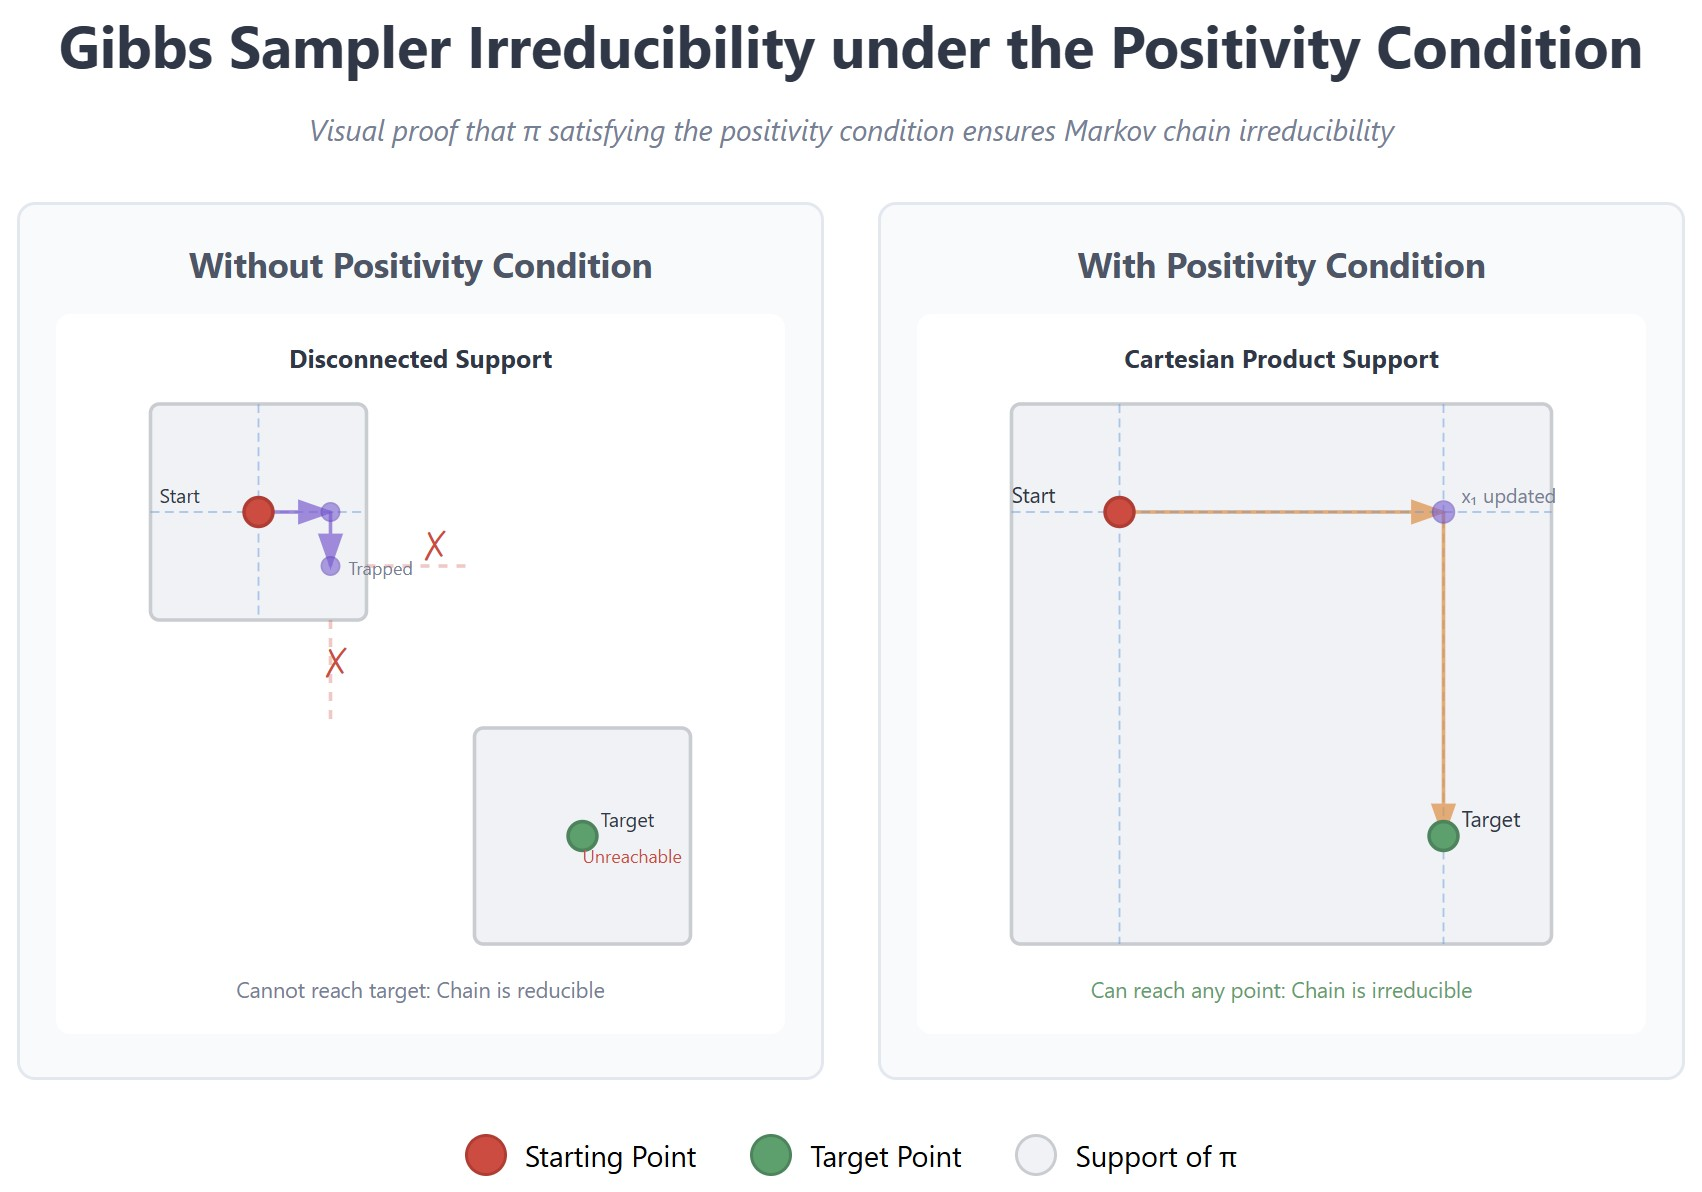
\includegraphics[width=0.8\textwidth]{positivity_condition.jpg}
		\caption{}
	\end{figure}
\end{frame}


\begin{frame}{$\pi$-irreducible}
	Assume $\pi$ satisfies the positivity condition, then the Gibbs sampler
	yields a $\pi$-irreducible Markov chain.

	\textbf{Irreducibility} Write $K$ for the transition kernel. We need to show that for
	any set $A \subset \mathbb{X}$ such that $\pi(A) > 0$, we have $K(x, A) > 0$ for
	any $x \in \mathbb{X}$. We have:
	\begin{equation*}
		K(x, A) = \int_A K(x, y)\,dy = \int_A \pi_{X_1|X_2}(y_1 \mid x_2) \times \pi_{X_2|X_1}(y_2 \mid y_1)\,dy_1dy_2
	\end{equation*}

	\textbf{Proof by contradiction:} Suppose that $K(x, A) = 0$ for some $A$ with $\pi(A) > 0$.
	Then we must have:
	\begin{equation*}
		\pi_{X_1|X_2}(y_1 \mid x_2) \times \pi_{X_2|X_1}(y_2 \mid y_1) = 0
	\end{equation*}
	for almost all $y = (y_1, y_2) \in A$.
\end{frame}

\begin{frame}{$\pi$-irreducible cont and Recurrence}
	By the Hammersley-Clifford theorem, the joint distribution satisfies:
	\begin{equation*}
		\pi(y_1, y_2) \propto \frac{\pi_{X_1|X_2}(y_1 \mid z_2)}{\pi_{X_1|X_2}(z_1 \mid z_2)} \times \frac{\pi_{X_2|X_1}(y_2 \mid y_1)}{\pi_{X_2|X_1}(z_2 \mid y_1)} = 0
	\end{equation*}
	for almost all $y = (y_1, y_2) \in A$.
	and hence implies $\pi(A) = 0$, which \textbf{contradicts} our assumption that $\pi(A) > 0$.

	\vspace{0.5cm}
	\textbf{Recurrence}: follows from irreducibility and the fact that $\pi$ is
	invariant (see Meyn and Tweedie, Proposition 10.1.1.)
\end{frame}

\begin{frame}{Convergence}
	Assume the Markov chain generated by the systematic scan Gibbs sampler is $\pi$-irreducible 
	and recurrent (both conditions hold when the positivity condition is satisfied) then we 
	have for any $\pi$-integrable function $\phi : \mathbb{X} \to \mathbb{R}$:
	\begin{equation*}
		\lim_{t \to \infty} \frac{1}{t} \sum_{i=1}^{t} \phi\left(X^{(i)}\right) = \int_{\mathbb{X}} \phi(x) \, \pi(x) \, dx
	\end{equation*}
	for $\pi$-almost all starting value $X^{(1)}$.
\end{frame}